\chapter{NDN node 23 - NTNU}\label{chp4:} 

\section{NDN node 23 - NTNU}
Node 23 in NDN testbed

\begin{figure}[ht]
  \centering
  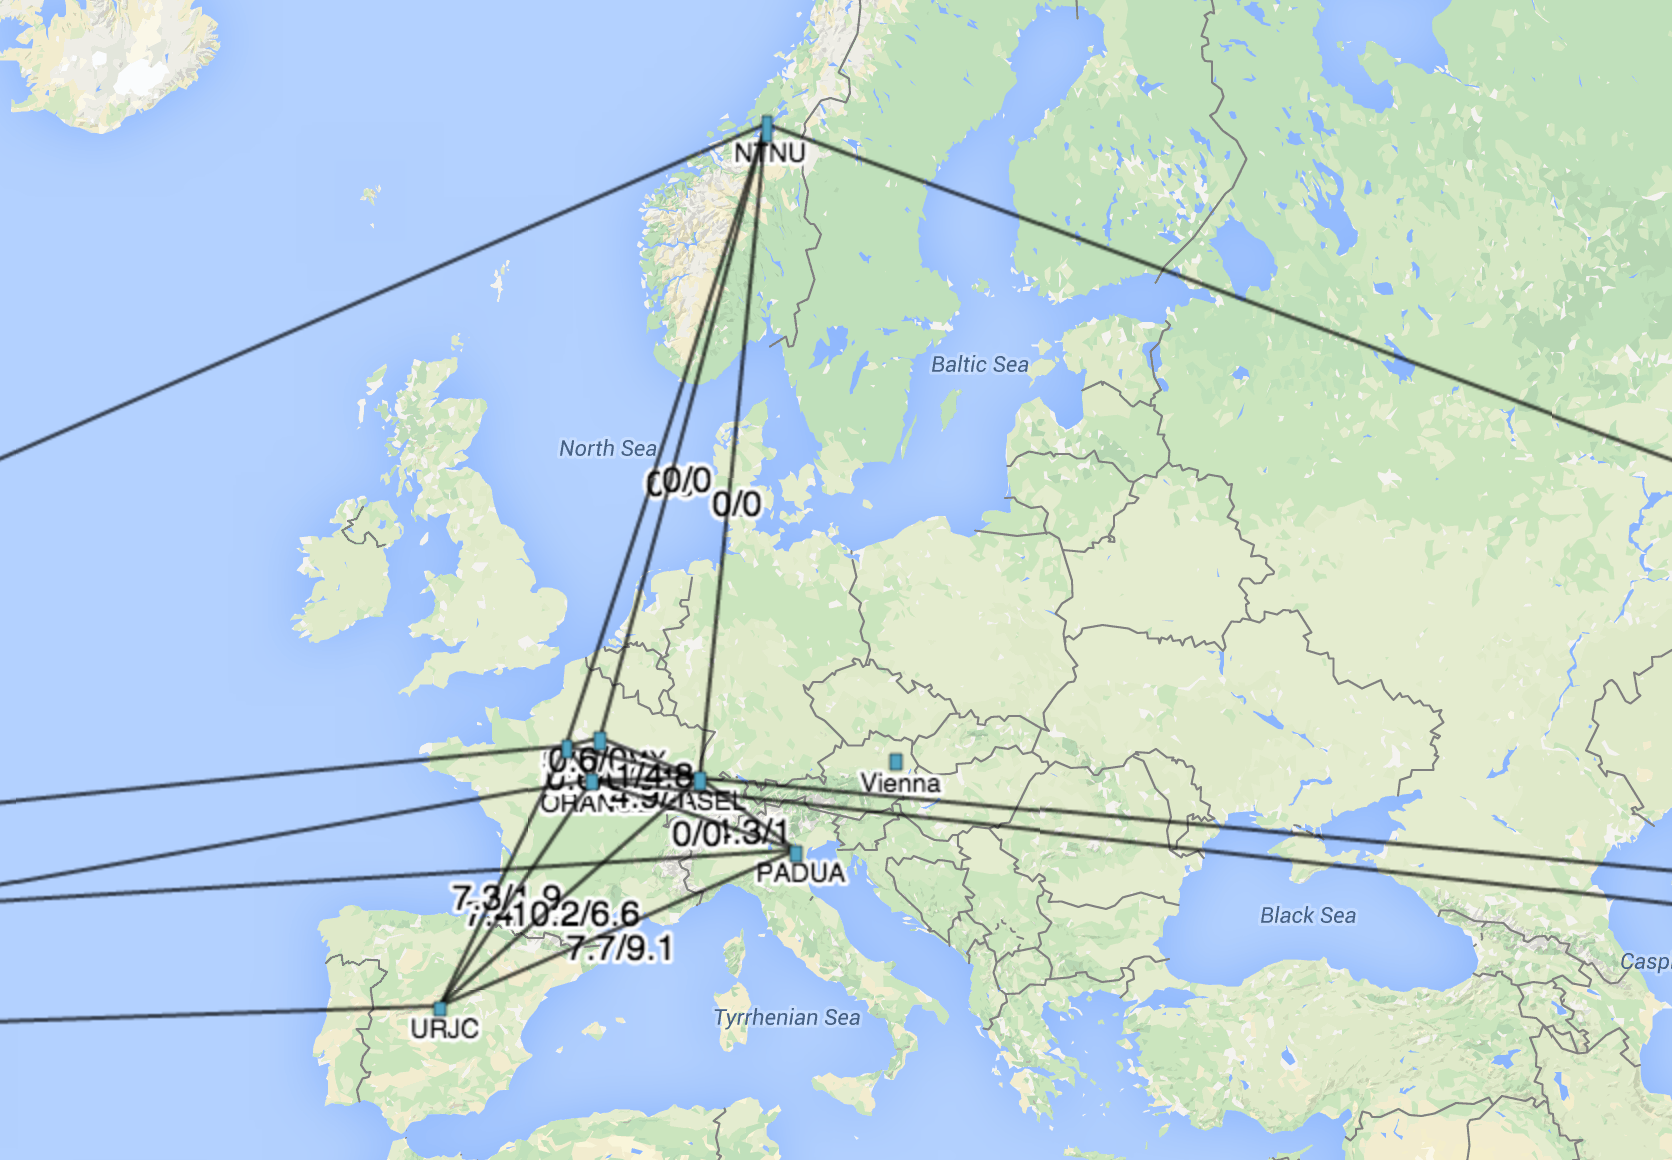
\includegraphics[width=1\textwidth]{ndn-map.png}
  \caption{NDN Map}
  \label{fig:ndn-map}
\end{figure}

\section{Public key distribution}
Instead of the PKI, where each pk is signed by a certificate authority and the generated certificate is sent as a response in https, then validated by the the client, we want to make the certificate authority obsolete by distributing every PK and rather trust the name (e.g. /ntnu/). 
